\documentclass[xetex,mathserif,serif, xcolor=table]{beamer}
\usepackage{polyglossia}
\setdefaultlanguage[babelshorthands=true]{russian}
\usepackage{minted}
\usepackage{tabu}
\usepackage{graphicx}
\usepackage{animate}


\newcommand*{\authorimg}[1]{%
  \raisebox{-.3\baselineskip}{%
    \includegraphics[
      height=\baselineskip,
      width=\baselineskip,
      keepaspectratio,
    ]{#1}%
  }%
}

\useoutertheme{infolines}

\usepackage{fontspec}
\setmainfont{FreeSans}
\newfontfamily{\russianfonttt}{FreeSans}

\definecolor{links}{HTML}{2A1B81}
\hypersetup{colorlinks,linkcolor=,urlcolor=links}

\setbeamertemplate{blocks}[rounded][shadow=false]
\setbeamercolor*{block title alerted}{fg=red!50!black,bg=red!20}
\setbeamercolor*{block body alerted}{fg=black,bg=red!10}

\tabulinesep=0.8mm

\title{Развлекательное приложение MemDer}
\author{Александр Смирнов и Феодор Жилкин}
\date{17.05.2019г}

\begin{document}

	\frame{\titlepage}

	\begin{frame}
		\frametitle{Введение}
		\begin{figure}[h]
            \center{\includegraphics[scale=0.095]{images/intro.png}}
            \caption{MemDer}
            \label{fig:image}
        \end{figure}
	\end{frame}
	
	\begin{frame}
		\frametitle{Цели}
			\begin{itemize}
		 		\item Сделать законченное Android-приложение
		 		    \begin{itemize}
    			    	\item Просмотр и оценка мемов
    			    	\item Общение между пользователями
    		    	\end{itemize}
		 		\item Выложить в Google Play
				\item Получение опыта
    				\begin{itemize}
    			    	\item Фронтенд
    			    	\item Бэкенд
    			    	\item Поиск и подбор контента
    			    	\item Сервер
    		    	\end{itemize}
			\end{itemize}
	\end{frame}
	
	\begin{frame}
		\frametitle{Задачи}
			\begin{itemize}
			    \item Скрипт по скачиванию контента
		 		\item База данных мемов по категориям
				\item Чаты
				\item Регистрация и вход пользователя
				\item Удобный интерфейс для просмотра мемов
				\item Уведомления о сообщениях
				\item Составление предпочтений пользователя
					\begin{itemize}
				    	\item Подбор собеседников по предпочтениям
				    	\item Подбор контента по предпочтениям
			    	\end{itemize}
			\end{itemize}
	\end{frame}	
	
	\begin{frame}
		\frametitle{Сравнение с аналогами}
			\begin{itemize}
				\item Текстовый развлекательный контент
					\begin{itemize}
				    	\item Пикабу
				    	\item Reddit
			    	\end{itemize}
			    \item Визуальный развлекательный контент
					\begin{itemize}
				    	\item Паблики с мемами в ВК
				    	\item iFunny
			    	\end{itemize}
			\end{itemize}
	\end{frame}		
	
	\begin{frame}
		\frametitle{Как это всё работает}
		\begin{figure}[h]
            \center{\includegraphics[scale=0.2]{images/scheme.png}}
            \caption{Схема проекта}
            \label{fig:image}
        \end{figure}
	\end{frame}	
	
	\begin{frame}
		\frametitle{Интерфейс приложения (1)}
            \begin{columns}[t]
                \column{.3\textwidth}
                    \includegraphics[scale=0.09]{images/login.png}
                \column{.3\textwidth}
                    \includegraphics[scale=0.179]{images/chats.png}
                \column{.3\textwidth}
                    \includegraphics[scale=0.09]{images/settings.png}
                    
            \end{columns}
	\end{frame}	
	
	\begin{frame}
		\frametitle{Пролистывание мемов}
		\begin{figure}[h]
		\begin{columns}[t]
		        \column{.5\textwidth}
                    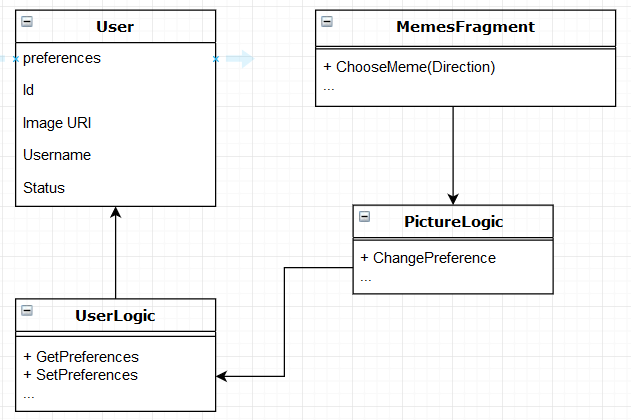
\includegraphics[scale=0.5]{images/swipe.png}
                    \caption{Логика свайпа}
                    \label{fig:image}
                \column{.2\textwidth}
                    \includegraphics[scale=0.09]{images/swipe1.png}
                    \caption{Свайп}
                    \label{fig:image}
            \end{columns}
        \end{figure}
	\end{frame}	
	
	\begin{frame}
		\frametitle{Рекомендательная система}
		     \begin{columns}[t]
                \column{.6\textwidth}
                    \begin{itemize}
                        \includegraphics[scale=0.179]{images/chats.png}
        			\end{itemize}
                \column{.3\textwidth}
                    \item Рекомендация контента
        		    \item Рекомендация пользователей
            \end{columns}
	\end{frame}	
	
	\begin{frame}
		\frametitle{Контентная фильтрация}
			\begin{itemize}
		    	\item Есть много контента – как выбрать наиболее подходящее?
		    	\item Предмет рекомендации – мемы из определенной категории (на самом деле категория)
		    	\item Пользовательские оценки получаем явно
		    	    \begin{itemize}
        		    	\item SuperLike = +2
        		    	\item SuperDislike = -2
        		    	\item Like = +1
        		    	\item Dislike = -1
        		    	\newline 
			        \end{itemize}
			      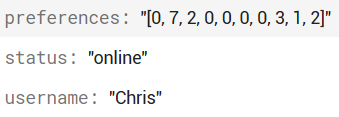
\includegraphics[scale=0.8]{images/user.png}   
			\end{itemize}
	\end{frame}
	
	
	\begin{frame}
	\frametitle{Контентная фильтрация}
        \begin{itemize}
            \item Среднее значение по вектору
            \item Байесовский классификатор
            \item Деревья решений
        \end{itemize}
	\end{frame}	
	
	\begin{frame}
	    \frametitle{Матрица предпочтений}
        \begin{table}[]
            \begin{tabular}{|c|c|c|c|c|}
                \hline
                \multicolumn{1}{|l|}{}                   & \cellcolor[HTML]{CBCEFB}Мемная папка & \cellcolor[HTML]{CBCEFB}4ch & \cellcolor[HTML]{CBCEFB}MDK & \cellcolor[HTML]{CBCEFB}Физкек \\ \hline
                \cellcolor[HTML]{CBCEFB}MemLover         & 9                                    & 5                           & 3                           & 8                              \\ \hline
                \cellcolor[HTML]{CBCEFB}Stepan           & 2                                    & 8                           & 6                           & 4                              \\ \hline
                \cellcolor[HTML]{CBCEFB}Д@nNJL           & 15                                   & 19                          & 13                          & 21                             \\ \hline
                \cellcolor[HTML]{CBCEFB}Polina\_Abramova & 7                                    & 9                           & 6                           & 7                              \\ \hline
            \end{tabular}
        \end{table}        
    \end{frame}		
	
	
	\begin{frame}
    	\frametitle{Фильтрация пользователей}
    	     \begin{itemize}
	            \item «Похожесть» или корреляцию предпочтений двух пользователей можно считать сравнением двух векторов предпочтений.
	         \end{itemize}
    	     \begin{columns}[t]
                \column{.4\textwidth}
                    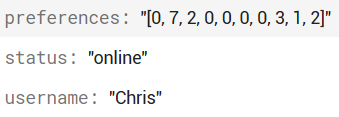
\includegraphics[scale=0.7]{images/user.png}
                \column{.4\textwidth}
                    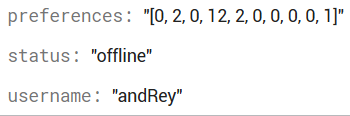
\includegraphics[scale=0.7]{images/user2.png}
            \end{columns}
	\end{frame}	

	\begin{frame}
	\frametitle{Фильтрация пользователей}
        \begin{itemize}
            \item Корреляция Пирсона
            \item Корреляция Спирмана
            \item Косинусное расстояние
                \begin{itemize}
                    \item Почему косинусное? 
                \end{itemize}
        \end{itemize}
	\end{frame}	
	
	
	\begin{frame}
	\frametitle{Фильтрация пользователей}
        \begin{itemize}
            \item Косинусное расстояние
            \newline
            {\Large $\mathbb \textbf{similarity} = cos(\theta) = \frac{AB}{|A||B|}= \frac{\sum\limits_{i=1}^n{A_iB_i}}{\sqrt{\sum\limits_{i=1}^n{A_i^2}}\sqrt{\sum\limits_{i=1}^n{B_i^2}}} $\par}
        \end{itemize}
	\end{frame}
	
	\begin{frame}
		\frametitle{Внутреннее устройство}
		\begin{figure}[h]
            \center{\includegraphics[scale=0.25]{images/diagram.png}}
            \caption{Диаграмма activity}
            \label{fig:image}
        \end{figure}
	\end{frame}	
	
	\begin{frame}
		\frametitle{FireBase FireStore}
		\begin{figure}[h]
            \center{\includegraphics[scale=0.5]{images/DB.png}}
            \caption{Схема БД}
            \label{fig:image}
        \end{figure}
	\end{frame}	
	
	
	\begin{frame}
		\frametitle{Итоги}
		     \begin{columns}[t]
                \column{.4\textwidth}
                    \begin{itemize}
                       \animategraphics[loop,controls,width=19ex]{6}{gif/gif-}{0}{82}
        			\end{itemize}
                \column{.4\textwidth}
                   \begin{itemize}
            			\item Александр
            			    \begin{itemize}
            			    	\item Чаты
            			    	\item FireStore
            			    	\item Буфер
            		        \end{itemize}
            			\item Феодор
            			    \begin{itemize}
            			    	\item Сбор контента
            			    	\item Рекомендательные системы  
            			    	\item Кастомные свайпы
		        \end{itemize}
		\end{itemize}
            \end{columns}		
	\end{frame}

	\begin{frame}
		\frametitle{Результаты}
		\begin{itemize}
		    \item Скрипт по скачиванию контента
			\item База данных мемов по категориям на FireBase
			\item Готовое Android-приложение, выложенное на Play Market
		    	\begin{itemize}
			    	\item Рекомендательная система для мемов
			    	\item Рекомендательная система для собеседников
			    	\item Дружелюбный интерфейс
			    	\item Чаты
			    	\item Регистрация/вход пользователя
			   	\end{itemize}
			\item Google Play — \url{https://play.google.com/store/apps/details?id=com.MemDerPack}
			\item Проект — \url{https://github.com/SmirnovAlexander/MemDer}
			\item Майнинг контента — \url{https://github.com/Feodoros/vkParser}
		\end{itemize}
	\end{frame}

\end{document}